% proci.tex

\cleardoublepage
\chapter{LODESTAR}\label{chapter:LODESTAR}


This chapter presents the package LODESTAR (Launch Optimisation and Data Evaluation for Scramjet Trajectory Analysis Research), which has been developed to calculate the optimal trajectories of partially airbreathing satellite launch systems, as a general tool for this purpose is not currently widely available. LODESTAR has the capability to calculate optimal mission profiles for systems consisting of various combinations of rocket and airbreathing stages, using \textcolor{red}{accurate and robust} optimisation techniques. 
LODESTAR optimises a trajectory towards a user-defined objective function, such as maximum payload-to-orbit, subject to constraints that ensure that the launch system does not exceed its aerodynamic or structural limitations.
LODESTAR calculates an optimal trajectory by simulating the dynamics of the launch system, and configuring an optimal control solver to define the launch trajectory optimisation problem being solved. 
The dynamics of the launch system are calculated in \textcolor{red}{three} degrees of freedom, with the performance of each vehicle calculated from aerodynamic and propulsion databases using precalculated interpolations, as described in Chapter \ref{chapter:Design}. These interpolations are designed to be smooth and continuous in order to improve the robustness of the optimal control solver.
LODESTAR separates a launch trajectory into multiple segments, to assist the solution process within the optimal control solver, improving robustness and accuracy. The segments with variable controls are solved within the optimal control solver, while the segments without control, or with prescribed control laws, are simulated directly in LODESTAR.
The segments which are simulated directly in LODESTAR are evaluated during the solution process, and the information necessary for the optimisation is passed to the optimal control solver.
Once the solution has been calculated, LODESTAR possesses the capability to verify the optimal control solution, an integral step when calculating an optimised trajectory with complex vehicle dynamics. 
LODESTAR is developed in MATLAB, and utilises GPOPS-2\cite{Patterson2015} as an optimal control solver. GPOPS-2 is a proprietary pseudospectral method optimisation package, which is based on an \textsf{hp}-adaptive version of the Radau pseudospectral method, described in further detail in Section \ref{sec:optsolvers}. 


 Within this chapter, the structure of LODESTAR is presented, as well as the set-up of LODESTAR for trajectory optimisation, and the verification methods used to determine if a solution has converged correctly.
 The configuration of LODESTAR presented in this chapter is designed specifically to calculate the maximum payload-to-orbit trajectory of a rocket-scramjet-rocket launch system, delivering a small satellite to sun synchronous orbit. 
 



\section{Mission Definition}\label{sec:mission}
The configuration of LODESTAR must be tailored towards the specific vehicle and mission profile which are being optimised. For this study, LODESTAR has been configured to simulate and optimise the launch of the rocket-scramjet-rocket vehicle, detailed in Chapter \ref{chapter:Design}, for maximum payload-to-orbit.
The nominal mission of the rocket-scramjet-rocket is presented here in order to provide a suitable reference for the configuration specifications, which are detailed in the following sections. 

The mission chosen for the optimal trajectory calculation is a launch to sun synchronous orbit. 
A satellite in sun synchronous orbit is at close to polar inclination, regressing so that it keeps its orbital alignment to the sun. The sun synchronous orbit is one of the most commonly used types of orbit for space science missions, as it has many useful properties\cite{Boain2004}. A sun synchonous orbit allows for global coverage, passing over each latitude at the same time each day, illustrated in Figure \ref{fig:SSO}. It also allows for a satellite to either have full sun and have consistent power generation, or alternatively, allows for a satellite to have a consistent `dark side' each day to alleviate thermal issues\cite{Boain2004}. A sun synchronous orbit at 566km has been used in previous studies as the target orbit\cite{Preller2017b}, and this orbit is also used for the current work. 
\begin{figure}[ht]
	\centering
	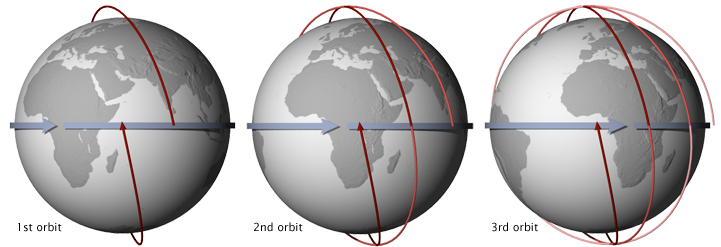
\includegraphics[width=0.8\linewidth]{figures/4_LODESTAR/SSO}
	\caption{Sun synchronous orbit illustration, passing over the equator at the same time each day\cite{NASASSO}.}
	\label{fig:SSO}
\end{figure}

The launch site selected for the simulation is the proposed Equatorial Launch Australia launch site near Nhulunbuy in the Northern Territory, Australia\cite{ELA}. This proposed launch site looks to take advantage of the remoteness of northern Australia, as well as its close proximity to the equator. While the proximity to the equator of this launch site is slightly disadvantageous for launch to sun synchronous orbits, the possibility of other launch directions from this location, and its active development, make it an appropriate choice as a practical launch location within Australia. The site is `about 30km south of Nhulunbuy'\cite{ELA} which places it within the approximate region indicated in Figure \ref{fig:SiteLocation}.

\begin{figure}[ht]
	\centering
	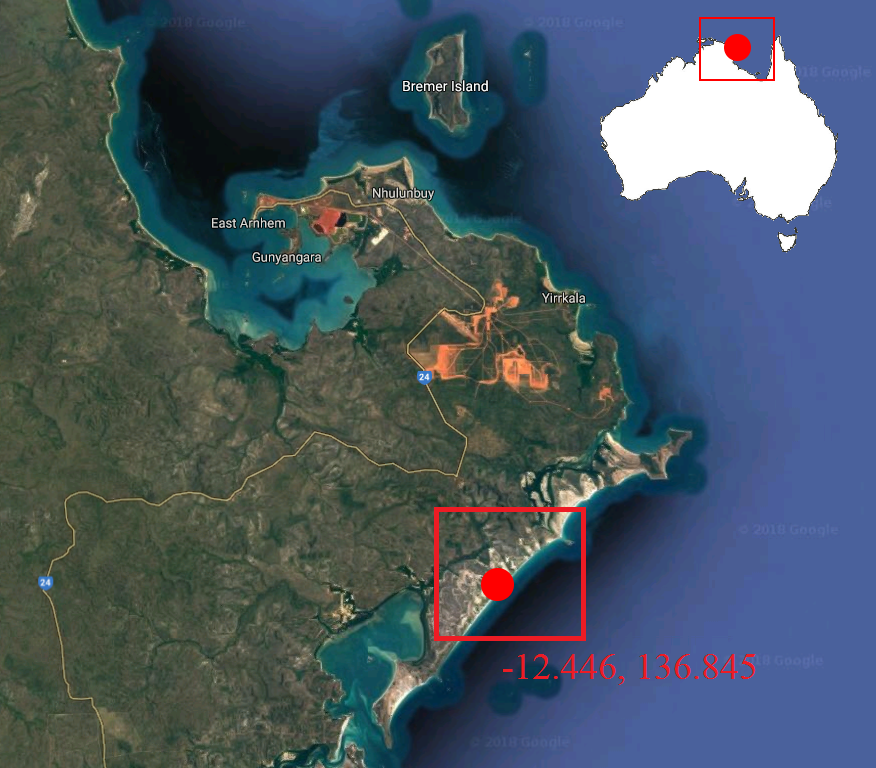
\includegraphics[width=0.7\linewidth]{figures/4_LODESTAR/SiteLocation}
	\caption{Approximate location of the ELA launch site. Image from Google maps.}
	\label{fig:SiteLocation}
\end{figure}


\section{Vehicle Simulation}

LODESTAR simulates each of the vehicles within the rocket-scramjet-rocket launch system by establishing a set of dynamic equations that fully describe the motion of the vehicle in terms of the time, states ($\mathbf{x}$), and controls ($\mathbf{u}$) of the system;
\begin{equation}\label{eq:states}
\dot{\textbf{x}}(t) = f[t,\textbf{x}(t),\textbf{u}(t)].
\end{equation}
 The states and controls are the variables that define the time dependent physical characteristics of the system. The state variables are dependent on the controls and the system dynamics, while the control variables drive the behaviour of the system and can be varied independently \cite{Stryk1992}.  
The state variables are defined by the coordinate system, and the outputs of each vehicle model \cite{Rao2009}. These are nonlinear functions, that depend on the interpolation of data sets which supply the atmospheric, aerodynamic, and propulsion characteristics of each vehicle. 
The methods used to interpolate these data sets must be as smooth and continuous as possible, and cover the entire possible operational range of the vehicle. 
Even if the optimal solution is well within the range of all input data sets, the optimal control solver will potentially explore all regions within the user-defined bounds. 
If there are large discontinuities or inaccurate extrapolation effects within the possible solution space of a particular vehicle, the solver may be unable to converge, or converge to a physically invalid solution. 
Discontinuities within the aerodynamics or engine properties of a particular vehicle must be mitigated through the careful application of interpolation techniques. Discontinuities that are unable to be mitigated, such as stage separations, must be separated into distinct phases within the optimal control solution and connected by linkage constraints \cite{Betts1998}, as discussed further in Section \ref{sec:optstruct}. 

\subsection{Equations of Motion}


The dynamics of the launch system are calculated in \textcolor{red}{three} degrees of freedom, in a geodetic rotational reference frame, illustrated in Figure \ref{fig:global}. The Earth is modelled as an ablate spheroid using the World Geodetic System 1984\cite{Icao2002} (WGS-84) shape and gravity model. In this reference frame, the dynamics of each vehicle are expressed in terms of the angle of attack $\alpha$, bank angle $\eta$, radius from centre of Earth $r$, longitude $\xi$, latitude $\phi$, flight path angle $\gamma$, velocity $v$ and heading angle $\zeta$. The equations of motion are given by\cite{Maddock2017,Tewari2007}:
\begin{figure}[ht]
	\centering
	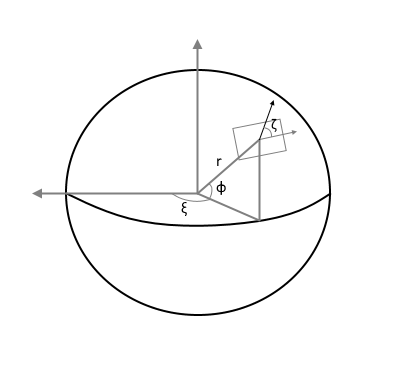
\includegraphics[width=0.7\linewidth]{figures/4_LODESTAR/global}
	\caption{The Earth-fixed components of the geodetic rotational coordinate system.}
	\label{fig:global}
\end{figure}


\begin{equation}
\dot{r} = v \sin \gamma
\end{equation}

\begin{equation}
\dot{\xi} = \frac{v\cos \gamma \cos \zeta}{r \cos \phi}
\end{equation}

\begin{equation}
\dot{\phi} = \frac{v\cos\gamma\sin\zeta}{r}
\end{equation}
\begin{equation}
\dot{\gamma} = \frac{(L + T\sin\alpha) \cos\eta}{mv} + (\frac{v}{r}-\frac{g_r}{v})\cos\gamma -\frac{g_t}{v}\sin\gamma\cos\zeta
+ \cos\phi[2\omega_E \cos\zeta + \frac{\omega_E^2 r}{v}(\cos\phi\cos\gamma+\sin\phi\sin\gamma\sin\zeta)]
\end{equation}
\begin{equation}
\dot{v} = \frac{T\cos\alpha - D}{m}-g_r\sin\gamma +g_t\cos\gamma\cos\zeta
+ \omega_E^2 r\cos\phi(\cos\phi\sin\gamma-\sin\phi\cos\gamma\sin\zeta)
\end{equation}
\begin{equation}\label{eq:heading}
\dot{\zeta} = \frac{(L + T\sin\alpha) \sin\eta}{mv \cos \gamma}-\frac{v}{r}\tan\phi\cos\gamma\cos\zeta +2\omega_E\cos\phi\tan\gamma\sin\zeta - \frac{\omega_E^2 r}{v\cos\gamma}\sin\gamma\cos\phi\cos\zeta-2\omega_E\sin\phi -g_t\sin\zeta
\end{equation}

Where $\omega_E$ is the angular velocity of the Earth, and $g_r$ and $g_t$ are the gravity of the Earth in the radial and transverse directions. These dynamics are used as the dynamic constraints of the launch system, as shown in Equation \ref{eq:states}, with each dynamic parameter implemented as a state variable ($\mathbf{x}$). The lift ($L$) and drag ($D$) forces are interpolated from the aerodynamic databases, described in Chapter \ref{chapter:Design}.

\section{Optimal Control Problem Structure}\label{sec:optstruct}

One of the primary functions of LODESTAR is to interface with the optimal control solver GPOPS-2. GPOPS-2 is a generic optimal control solver that utilises the pseudospectral method of optimal control, as well as the IPOPT nonlinear optimisation package. GPOPS-2 is described in detail in Section \ref{sec:optsolvers}. Practically, the implementation of optimal control involves the specification of the dynamics of the system to be optimised, as well as the set of constraints and objectives that define the optimisation problem, described as follows:

\noindent \textit{Cost Function}

\noindent The cost function, $J$, defines the target of the optimisation problem. 
This cost function may be any function which is defined by the states or controls of the optimisation problem. The cost function is defined as follows:
\begin{equation} \label{eq:cost}
J(t,\textbf{x}(t),\textbf{u}(t)) = M[t,\textbf{x}(t_f),\textbf{u}(t_f)] +   \int_{t_0}^{t_f} P[\textbf{x}(t),\textbf{u}(t)] dt, \quad t \in [t_0,t_f],
\end{equation}
where $M$ is the terminal cost function and $P$ is the time integrated cost. 

\noindent \textit{Dynamic Constraints}

\noindent 
The optimisation problem is subject to a set of dynamic constraints, which describe the behaviour of the system over the solution space:
\begin{equation} \label{eq:state}
\dot{\textbf{x}}(t) - f[t,\textbf{x}(t),\textbf{u}(t)] = 0, \quad t \in [t_0,t_f].
\end{equation}
These dynamic constraints ensure that the polynomial approximations of the state variables, as described in Section \ref{sec:PS}, match the physical dynamics of the system. Implementing the dynamics as constraints in the manner of the pseudospectral method allows each state variable to be approximated separately, and gives the optimiser some freedom to explore each state variable independently, greatly increasing the robustness of the optimal control problem.



\noindent \textit{Bounds and Path Constraints}

\noindent Inequality constraints define the bounds of each state, as well as any path constraints.
The bounds directly confine the state and control variables to prescribed values. This serves the purpose of limiting the search space to the physically possible (eg. constraining altitude to be greater than ground level), constraining the vehicle within its performance limits (eg. limiting the angle of attack), and improving computational efficiency by ensuring that the optimiser is constrained to a reasonable solution space:
\begin{eqnarray}
\mathbf{b}_{min} \leq \textbf{x}(t),\textbf{u}(t) \leq \mathbf{b}_{max}, \quad t \in [t_0,t_f].
\end{eqnarray}
The path constraints are inequality constraints which consist of functions based on the states and controls of the system. Path constraints place adaptive bounds on the system, which vary over time with the state of the system:
\begin{eqnarray}
\mathbf{\lambda}[t,\textbf{x}(t),\textbf{u}(t)] \leq \textbf{0}, \quad t \in [t_0,t_f].
\end{eqnarray}
Path constraints are used by LODESTAR to impose physical limitations on the system such as structural, aerothermodynamic, pathing, and control limits.

\noindent \textit{Event Constraints}

\noindent The event constraints constrain the states at the start and end points of a trajectory or phase:
\begin{equation}
\mathbf{\psi}_0[\textbf{x}(t_{0}), t_{0}] = \textbf{0},
\end{equation}
\begin{equation} \label{eq:2}
\mathbf{\psi}_f[\textbf{x}(t_{f}), t_{f}] = \textbf{0}.
\end{equation}
These constraints determine the initial and terminal conditions of the optimisation problem, such as the initial location and velocity, and the starting fuel mass.


Together, these objectives, constraints, and variables describe the optimal control problem being solved, and form the inputs which LODESTAR provides to GPOPS-2. GPOPS-2 uses these inputs, along with a pseudospectral method transcription, to form the constrained optimisation problem that is solved using IPOPT.









\subsection{Trajectory Connection Points}
The optimisation of a large, multi-vehicle launch trajectory requires that the optimal control problem be broken down into multiple segments, or phases\cite{Patterson2015}.
 These phases are joined by event constraints, which couple the states and time of each phase to the preceding and following phases as follows:
 \begin{equation}\label{eq:cont1}
 \textbf{x}_{f,1} - \textbf{x}_{0,2} = 0,
 \end{equation}
 \begin{equation}\label{eq:cont2}
 \textbf{t}_{f,1} - \textbf{t}_{0,2} = 0.
 \end{equation}
 This segmentation is performed in order to assist the convergence of the optimal control solver, by ensuring that the dynamics of the underlying model are as smooth and continuous as possible across each segment. 
  \begin{figure}[ht]
  	\centering
  	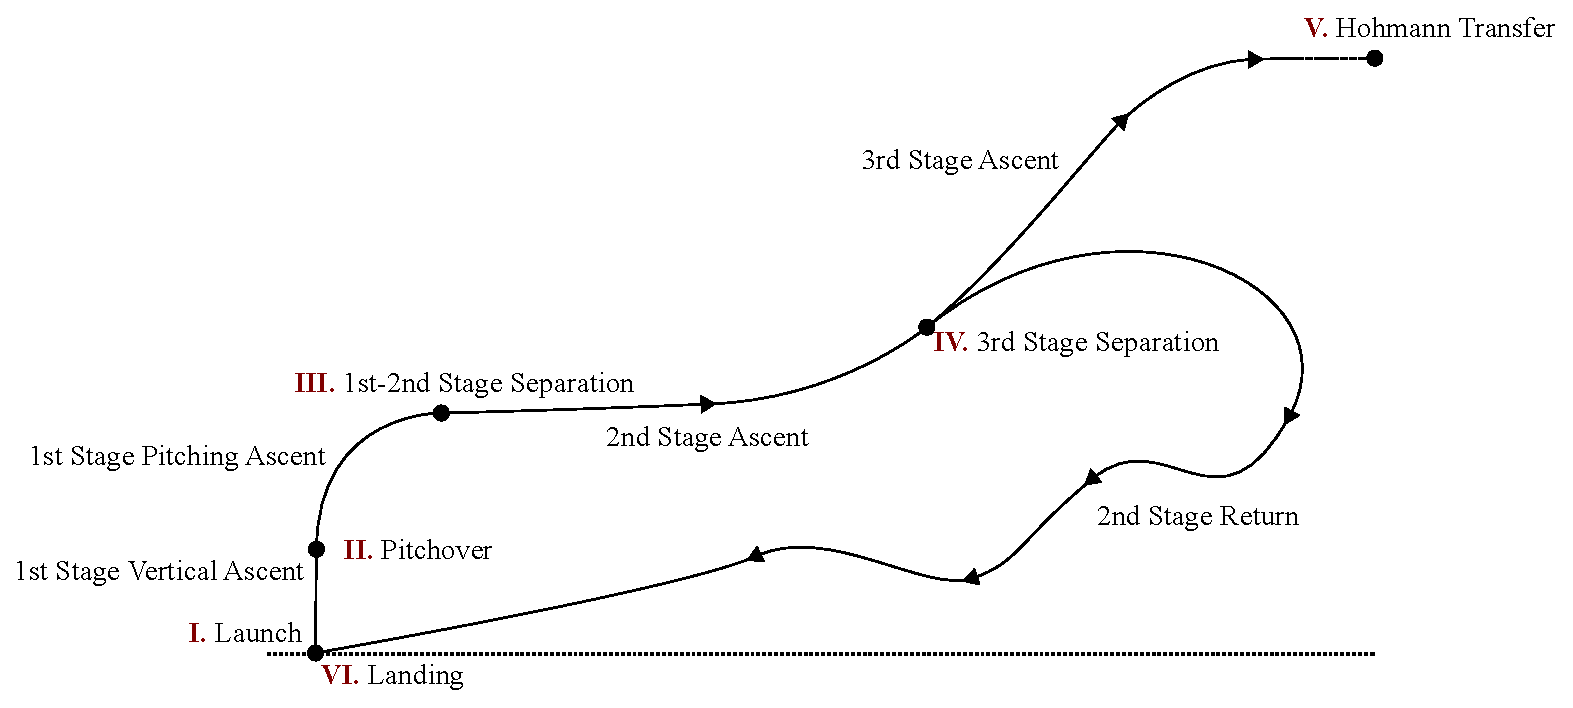
\includegraphics[width=1.\linewidth]{figures/4_LODESTAR/Traj}
  	\caption{Illustration of the phases of the launch profile. Controlled and uncontrolled phases are distinguished. }
  	\label{fig:Traj}
  \end{figure}
  
For a launch system, discontinuities in the system dynamics generally arise when the aerodynamics, mass or propulsion mode of a launch vehicle change significantly between stages or flight modes. 
If a vehicle model with large discontinuities is implemented directly into a single phase application of the pseudospectral method, it is likely to cause significant convergence issues, as the system dynamics will be unable to be approximated by the underlying polynomial of the pseudospectral method across these transition points\cite{Betts2009}.

 
 To allow the trajectory profile to be formulated as an optimal control problem, the trajectory of the rocket-scramjet-rocket launch system is broken down into the seven segments shown in Figure \ref{fig:Traj}. 
  The segments are separated into two groups; controlled segments which take the form of phases within the optimal control problem; and segments without control which are either forward simulated at each iteration of the optimiser, or simulated externally to the optimal control problem. The unpowered segments of the third stage are simulated within the optimiser, and are included as a terminal cost, as described in Equation \ref{eq:cost}. 
  
 Segments \textcolor{red}{\rom{2}-\rom{5}} are controlled by various combinations of angle of attack, bank angle and throttle, and are implemented as the phases of the optimisation problem. These phases are: \textcolor{red}{\rom{2}}, the 1st stage pitching ascent; \textcolor{red}{\rom{3}}, the 2nd stage ascent; \textcolor{red}{\rom{4}}, the 2nd stage return flight; and \textcolor{red}{\rom{5}}, the 3rd stage powered ascent.
 Segments \textcolor{red}{\rom{1}},\textcolor{red}{\rom{6}} and \textcolor{red}{\rom{7}} are segments without direct control, which are simulated using forward time stepping methods. 
 These phases are: the pre-pitch segment of the first stage, the unpowered section of the third stage ascent, and the final Hohmann transfer to orbit. 
 Each segment is connected through a set of continuity constraints. 
  The optimal control problem phases are connected through the use of initial and end discontinuity constraints (Equations \ref{eq:cont1} and \ref{eq:cont2}), while the forward simulated segments are simply initiated and terminated at set conditions. 
 The segment coupling conditions are described in Table \ref{tab:constraints}.


The following sections describe the setup of each individual phase of the optimal control problem, including the variables and constraints for the optimised phases. 
The bounds on the state dynamics are chosen to encompass the solution space, while not being overly expansive, to assist with the convergence and scaling of the optimal control solver. 
Across all optimised phases, the bounds on the latitude and longitude are chosen to cover the possible solution space, and are kept consistent across each phase to ensure that the position of the vehicle is not being unreasonably constrained between segments. The velocity constraints are chosen to cover the possible solution space, with the lower bound of 10m/s chosen to ensure that the velocity does not approach 0m/s, as this produces singularities within the system dynamics.




\begin{table}[ht]


\begin{tabularx}{\linewidth}{|X|X|X|c|}
	\hline \textbf{Section} & Initial Conditions & End Conditions & Controlled \\ 
	\hline \textcolor{red}{\rom{1}}: $1^{st}$ Stage Vertical Ascent  & Launches from rest, at the predefined launch site. & Fly until pitchover conditions are met. & no \\ 
	\hline \textcolor{red}{\rom{2}}: $1^{st}$ Stage Pitching Ascent  & Start at pitchover conditions & Terminates at end of fuel. & yes\\ 
	\hline \textcolor{red}{\rom{3}}: $2^{nd}$ Stage Ascent  & Must begin at $1^{st}$ stage pitching ascent end conditions. & Terminates at end of ascent fuel. & yes\\ 
	\hline \textcolor{red}{\rom{4}}: $2^{nd}$ Stage Return  & Must begin at $2^{nd}$ stage ascent end conditions. & Must approach landing conditions at the initial launch site. & yes\\ 
	\hline \textcolor{red}{\rom{5}}: $3^{rd}$ Stage Powered Ascent  & Must begin at $2^{nd}$ stage ascent end conditions.  & Must produce exoatmospheric flight at the termination of stage \rom{6}.  & yes\\ 
	\hline \textcolor{red}{\rom{6}}: $3^{rd}$ Stage Unpowered Ascent  & Must begin at $3^{nd}$ stage powered ascent end conditions.  & Terminates when flight is parallel with Earth's surface.  & no\\ 
	\hline \textcolor{red}{\rom{7}}: $3^{rd}$ Stage Hohmann Transfer  & Must begin at $3^{rd}$ stage unpowered ascent end conditions. & Must attain prescribed orbit.  & no\\ 
	\hline 
	
\end{tabularx} 
\caption{Segment coupling conditions for combined trajectory optimisation.}
\label{tab:constraints}

\end{table}



\subsection{\textcolor{red}{\rom{1}.} First Stage Vertical Ascent}

LODESTAR optimises the ascent of the first stage rocket in two segments; pre and post-pitchover.
 These aerodynamics of flight during these segments are simulated using spline interpolation of the databases generated using the method described in Section \ref{sec:firststageaero}, and the engine properties are determined using linear pressure scaling as described in Section \ref{sec:firststage}. 
  
 The pre-pitchover phase is the segment of flight immediately after vertical launch. During this phase, the launch system continues vertically for a short time in order to clear the launch tower and stabilise the vehicle.        
The pre-pitchover section is prescribed, and is simulated externally to the optimisation to allow the dynamics of the system to behave appropriately during the pitching ascent. During vertical flight, the heading angle (Equation \ref{eq:heading}) is meaningless, and vertical flight is allowed during the pitching ascent, the heading angle change rate can tend towards infinity, causing mathematical and scaling errors. Simulating this segment after the optimisation has been completed makes the starting mass and altitude of the first stage slightly variable, but this variation is negligible. 
The pitchover is defined to occur at 30m altitude and 15m/s velocity.
During the vertical launch the rocket is assumed to need no control, and is held at 0$^\circ$ angle of attack. 

\subsection{\textcolor{red}{\rom{2}.} First Stage Pitching Ascent}

\begin{table}[ht]
	\centering
	\begin{tabular}{|c|c|c|}
		\hline \textbf{Variable Group}  & \textbf{Associated Variables} & \textbf{Value/Range}\\
		\hline Initial Constraints  & Velocity (v) & 30m/s\\ & Altitude (z)& 30m \\ & Latitude ($\phi$)  & $-12.16^\circ$ \\& Longitude ($\xi$) & 136.75$^\circ$\\ & Trajectory Angle ($\gamma$) & 89.9$^\circ$\\ & Angle of Attack ($\alpha$)& 0$^\circ$\\
		\hline Terminal Constraints & $\textbf{x}_{f,\textrm{\rom{2}}} - \textbf{x}_{0,\textrm{\rom{3}}}$ & 0\\ & $t_{f,\textrm{\rom{2}}} - t_{0,\textrm{\rom{3}}}$ & 0\\
		\hline Path Constraints & Dynamic Pressure ($q$) & 0kPa - 50kPa\\ 
		\hline Control Variables & $\ddot{\alpha}$ & $\pm0.029^\circ/s^2$\\ 
		\hline State Variables & Altitude (z) & 0 - 30km\\ & Velocity (v) & 10 - 3000m/s\\ & Trajectory Angle ($\gamma$)& $-5.7^\circ$ - $89.9^\circ$ \\   & Latitude ($\phi$) & $\pm28.6^\circ$ \\  & Longitude ($\xi$)& $114.6^\circ$ - $171.9^\circ$\\   & Heading Angle ($\zeta$)& $\pm360^\circ$\\  & Total Mass (m)& 11453 - 29388kg \\  & Angle of Attack ($\alpha$)&  $-5^\circ$ - 0$^\circ$\\  & $\dot{\alpha}$& $\pm5.7^\circ/s$\\ 
		\hline 
	\end{tabular} 
	
	\caption{Optimisation setup of the first stage phase. }
	\label{tab:1ststagesetup}
\end{table}


At 30m altitude and 15m/s velocity, pitchover occurs. The pitchover is a very minor amount of instantaneous pitching (0.01$^\circ$) which is introduced in order to begin the pitching ascent, allowing the heading angle of the vehicle to resolve correctly. 
The first stage pitching ascent trajectory is an angle of attack controlled phase in the optimisation routine, which is simulated from pitchover until second stage separation. Table \ref{tab:1ststagesetup} shows the optimisation setup of this phase. During this phase, the launch system is allowed to fly at negative angles of attack, to assist in pitching. The control for this phase is the second derivative of angle of attack, which is chosen as the control variable to assist in mitigating the first stage's sensitivity to angle of attack, ie. when the trajectory angle is near 90$^\circ$ and at low velocities, the effects of changes in angle of attack on the dynamics of the system are very large. This sensitivity can cause convergence issues, which are mitigated by using the second derivative of angle of attack as the control variable. 
The initial fuel mass of the first stage rocket is not fixed, as variations in the initial fuel mass can have an important effect on the capabilities of the first stage. The fuel mass can influence the velocity achievable at first to second stage separation, as well as the rate at which the rocket is able to pitch, and consequentially, the altitude and flight path angle range of the first stage.
Allowing the initial fuel mass to vary increases the flexibility of the optimal control solver, and enables the optimal sizing of the first stage to be investigated. 



\subsection{\textcolor{red}{\rom{3}.} Second Stage Ascent Trajectory}


\begin{table}[ht]
	\centering
	\begin{tabular}{|c|c|c|}
		\hline \textbf{Variable Group}  & \textbf{Associated Variables} & \textbf{Value/Range}\\
		\hline Initial Constraints  & Fuel Mass ($m_F$) & 1562kg\\ 
		Terminal Constraints & $\textbf{x}_{f,\textrm{\rom{2}}} - \textbf{x}_{0,\textrm{\rom{3}}}$ & 0\\ & $t_{f,\textrm{\rom{2}}} - t_{0,\textrm{\rom{3}}}$ & 0\\
		\hline Terminal Constraints & Altitude (z) & 0 - 45km\\ & Trajectory Angle ($\gamma$)& 0 - 15$^\circ$\\  & Bank Angle ($\eta$)& 0$^\circ$\\  & $\textbf{x}_{f,\textrm{\rom{3}}} - \textbf{x}_{0,\textrm{\rom{4}}}$ & 0\\ & $t_{f,\textrm{\rom{3}}} - t_{0,\textrm{\rom{4}}}$ & 0\\
		 & $\textbf{x}_{f,\textrm{\rom{3}}} - \textbf{x}_{0,\textrm{\rom{5}}}$ & 0\\ & $t_{f,\textrm{\rom{3}}} - t_{0,\textrm{\rom{5}}}$ & 0\\
		\hline Path Constraints & Dynamic Pressure& 0 - 50kPa\\ 
		\hline Target Cost (Optional) & Dynamic Pressure$^*$ & $(q-50000)^2/50000$\\ 
		\hline Control Variables & $\dot{\alpha}$ &  $\pm0.5^\circ$/s\\  & $\dot{\eta}$ &  $\pm1^\circ$/s\\ 
		\hline State Variables & Altitude (z) & 0 - 50km\\ & Velocity (v)& 10 - 3000m/s\\ & Trajectory Angle ($\gamma$)& $-28.6^\circ$ - $15^\circ$\\   & Latitude ($\phi$) &$\pm28.6^\circ$ \\  & Longitude ($\xi$)& $114.6^\circ$ - $171.9^\circ$\\   & Heading Angle ($\zeta$)& $-240^\circ$ - $360^\circ$ \\  & Fuel Mass ($m_F$)& 0 - 1562kg \\  & Angle of Attack ($\alpha$)&  0$^\circ$ - $10^\circ$ \\  & Bank Angle $\eta$& $-1^\circ$ - $90^\circ$ \\  
		\hline 
	\end{tabular} 
	\caption{Optimisation setup of the second stage ascent. $^*$ This is only used in the constant dynamic pressure simulation. \textcolor{red}{XXX Check these, particularly traj angle}}
	\label{tab:SPARTANascentsetup}
\end{table}

The second stage ascent phase consists of the acceleration of the SPARTAN scramjet-powered vehicle, controlled using the SPARTAN's angle of attack and bank angle. The optimisation setup of this phase is detailed in Table \ref{tab:SPARTANascentsetup}.
The propulsion, lift, and drag of the vehicle are obtained from interpolation of the C-RESTM10 and trimmed aerodynamics databases described in Sections \ref{sec:propulsion}, \ref{sec:trimmedongineon}, and \ref{sec:trimmedongineoff}. 
During the ascent, the engines are assumed to be operating at the maximum thrust, corresponding to the maximum equivalence ratio at all times. This equivalence ratio is 1 in most sections of the trajectory, except at low Mach numbers where the possibility of unstart and choking necessitates a reduction in equivalence ratio. This trajectory is constrained by a maximum dynamic pressure of 50kPa, corresponding to the maximum structural limits of the vehicle. 
The control variables are set as the rate of change of angle of attack, and the rate of change of bank angle. Using the derivatives of the angle of attack and bank angle as the control variables serves to smooth the angle of attack and bank angle by constraining the change rates. The angle of attack is constrained to 10$^\circ$, approximated as a reasonable upper bound to the angle of attack, and the limit to which the aerodynamic characteristics of the SPARTAN are modelled. The bank angle is constrained to a maximum of 90$^\circ$, as it is assumed that the SPARTAN is not able to invert. The bank angle is also constrained to positive values only (ie. the heading angle may only increase) as the SPARTAN is launched from the ELA launch site at Nhulunbuy, and it is preferable to launch to the northeast or east to avoid overflying populated areas. 

A cost function can be included during this phase, shown in Table \ref{tab:SPARTANascentsetup}, when flying a constant dynamic pressure trajectory is desired. This cost function is smooth and approaches 0 at the target dynamic pressure, allowing the third stage cost function of payload mass to still be active, while prioritising flying at constant dynamic pressure. 


\subsection{\textcolor{red}{\rom{4}.} Second Stage Return Trajectory}

\begin{table}[ht]
	\centering
	\begin{tabular}{|c|c|c|}
		\hline \textbf{Variable Group}  & \textbf{Associated Variables} & \textbf{Value/Range}\\
		\hline Initial Constraints  & Bank Angle ($\eta$)& 0$^\circ$ \\ 
		& $\textbf{x}_{f,\textrm{\rom{3}}} - \textbf{x}_{0,\textrm{\rom{4}}}$ & 0\\ & $t_{f,\textrm{\rom{3}}} - t_{0,\textrm{\rom{4}}}$ & 0\\
		\hline Terminal Constraints& Latitude ($\phi$)  & $-12.16^\circ$ \\& Longitude ($\xi$) & 136.75$^\circ$\\
		\hline Path Constraints & Dynamic Pressure ($q$)& 0 - 50kPa\\ 
		\hline Control Variables & $\dot{\alpha}$ &  $\pm0.5^\circ$/s\\  & $\dot{\eta}$ &  $\pm1^\circ$/s\\ & $\dot{Throttle}$& $\pm0.2$/s\\
		\hline State Variables& Altitude (z) & 0 - 70km\\ & Velocity (v)& 10 - 5000m/s\\ & Trajectory Angle ($\gamma$)& $\pm80^\circ$\\    & Latitude ($\phi$) &$\pm28.6^\circ$ \\  & Longitude ($\xi$)& $114.6^\circ$ - $171.9^\circ$\\   & Heading Angle ($\zeta$)& $60^\circ$ - $500^\circ$ \\  & Fuel Mass ($m_F$)& 0kg - 500kg\\  & Angle of Attack ($\alpha$)&  0$^\circ$ - 10$^\circ$\\  & Bank Angle ($\eta$)& $0^\circ$ - 90$^\circ$\\  & Throttle & 0 - 1 \\ 
		\hline 
	\end{tabular} 
	\caption{Optimisation setup of the second stage return.}
	
\end{table}

After releasing the third stage rocket, the scramjet-powered second stage must return back to the initial launch site. During this return flight, the SPARTAN is able to use its engines if necessary to ensure that it is able to return successfully. 
During the fly-back, the SPARTAN cannot exceed its dynamic pressure limit of 50kPa. 
 The end state is constrained to a minimum of $-20^\circ$ trajectory angle, which is assumed to be an appropriate lower bound on the trajectory angle for approach to a landing strip. The altitude is constrained to less than 1km at the end point to ensure that the SPARTAN is approaching landing altitude.
 The velocity at the termination of the return trajectory is left variable. Constraining the end velocity may over-constrain the optimisation problem, and it is assumed that for a payload-to-orbit optimised trajectory the SPARTAN will end its return at a low velocity, so that the energy necessary for return is minimised. 
 
 
 
 The aerodynamics of the SPARTAN during fly-back are determined by interpolation of the engine-on and engine-off trimmed data sets described in Section \ref{sec:aero}.
During the return, the C-REST engines are able to be throttled on and off. 
 As the scramjet engines are throttled on, the aerodynamics are assumed to vary linearly between the aerodynamics calculated by the engine-off and engine-on datasets. 
The throttle setting is defined as a state variable, with range between 0 and 1, where 1 represents the maximum equivalence ratio at that point. The corresponding fuel mass flow rate is scaled linearly with the throttle:  
\begin{equation}
\dot{m}_{fuel} = \dot{m}_{fuel,max}throttle,
\end{equation}
and the thrust of the engine is assumed to scale linearly with the fuel mass flow rate. A control variable of throttle change rate is added, to smooth the throttle in the same way as angle of attack and bank angle. 

 

\subsection{\textcolor{red}{\rom{5}.} Third Stage Powered Ascent}


\begin{table}[ht]
	\centering
	\begin{tabular}{|c|c|c|}
		\hline \textbf{Variable Group}  & \textbf{Associated Variables} & \textbf{Value/Range}\\	\hline Initial Constraints  & Total Mass (m) & 3300kg\\ 
		& $\textbf{x}_{f,\textrm{\rom{3}}} - \textbf{x}_{0,\textrm{\rom{5}}}$ & 0\\ & $t_{f,\textrm{\rom{3}}} - t_{0,\textrm{\rom{5}}}$ & 0\\
		\hline Terminal Constraints & Alt$_{f,\textrm{\rom{6}}}$ & $\geq$90km\\ & Heading Angle ($\zeta$) $_{\textrm{\rom{6}}}$ & 97.64$^\circ$\\  & Angle of Attack ($\alpha$) & 0$^\circ$\\
		\hline Path Constraints & Angle of Attack ($\alpha$) & Maximum $F_N$\\  & Thrust Vector Angle & $\pm8^\circ$\\ 
		\hline Target Cost & Payload-to-Orbit & Payload Calculated in Phase \rom{7}\\ 
		\hline Control Variables & $\dot{\alpha}$ & $\pm1^\circ$\\ 
		\hline State Variables & Altitude (z) & 30 - 84km\\ & Velocity (v)& 10 - 8000m/s\\ & Trajectory Angle ($\gamma$)& $-5^\circ$ - 30$^\circ$ \\   & Latitude ($\phi$) &$\pm28.6^\circ$ \\   & Heading Angle ($\zeta$)& $80^\circ$ - 120$^\circ$\\  & Total Mass (m)& 0kg - 3300kg \\  & Angle of Attack ($\alpha$)&  $-5^\circ$ - 0$^\circ$\\ 
		\hline 
	\end{tabular} 
	\caption{Optimisation setup of the third stage powered ascent.}
	\label{tab:thirdstageopt}
\end{table}

The trajectory of the third stage rocket is separated into the powered and unpowered phases of ascent.
During the powered ascent phase, the third stage is manoeuvred out of the atmosphere using one continuous burn of the Kestrel engine. The powered ascent is an optimised phase, with optimisation properties described in Table \ref{tab:thirdstageopt}. 
 The powered phase is controlled using angle of attack, and trimmed using thrust vectoring of the engine, as described in Section \ref{sec:thrustvectoring}. The aerodynamics of the third stage are determined using interpolation of the aerodynamic dataset developed as described in Section \ref{sec:thirdstageaero}.

The third stage rocket is constrained to an angle of attack of less than 20$^\circ$. This is assumed to be the maximum controllable angle of attack possible for the third stage rocket.   
Additionally, a maximum normal force restriction is placed on the third stage, to limit the angle of attack of the third stage by the normal force on the vehicle. However, as a detailed structural study of the third stage has not been conducted, the maximum allowable normal force on the third stage is not certain.
For consistency, the maximum allowable normal force was calculated from the conditions of previous studies. Previous studies flew the third stage rocket at a constant 10$^\circ$ angle of attack, and initially released the rocket at 50kPa\cite{Preller2017b}. 
It is assumed that these release conditions produce the maximum allowable normal force on the third stage rocket. The maximum allowable normal force is calculated at the release Mach number, and is set as a path constraint. 

The end angle of attack is constrained to 0$^\circ$, as the angle of attack will not be able to be controlled during the unpowered ascent. 
The other terminal constraints of this phase correspond to end constraints imposed after the third stage unpowered ascent has been simulated. The altitude at the end of the unpowered ascent (Phase \textcolor{red}{\rom{6}}) is constrained to a lower limit of 90km, in order to ensure that the rocket is exoatmospheric. The final heading angle is also constrained at this point, so that the orbit of the third stage attains the correct inclination for sun synchronous orbit. 


\subsection{\textcolor{red}{\rom{6}.} Third Stage Unpowered Ascent}
After the burn of the Kestrel engine is complete, at the end of phase \textcolor{red}{\rom{5}}, the engine is cut and the third stage coasts to exoatmospheric conditions. 
The unpowered phase of the ascent is not controlled. After the engine is cut, the third stage does not have sufficient aerodynamic control to manoeuvre, and the trajectory of the third stage is a coast at 0$^\circ$ angle of attack. The trajectory of the third stage rocket is only directly optimised during the powered section of its trajectory, the unpowered section of the trajectory is simulated from the end of the controlled section of the trajectory, using a second order Taylor series approximation. This integration ceases when the flight path angle reaches 0$^{\circ}$.
During this phase, the heat shield is released once the rocket has reached a dynamic pressure of 10Pa, where it is assumed that atmospheric effects will have ceased to have a major thermal effect.  As the third stage is required to deliver the payload into heliosynchronous orbit, the third stage must achieve an inclination of 97.63$^\circ$ at the end of this phase\cite{Boain2004}. These terminal constraints are implemented in Phase \textcolor{red}{\rom{5}}.



\subsection{\textcolor{red}{\rom{7}.} Hohmann Transfer}
After the rocket has attained exoatmospheric flight parallel to the Earth's surface, a circularisation burn is performed. This circularisation burn takes the third stage rocket into low orbit around the Earth. 
However, in order to reach a heliosynchronous orbit of 567km, the orbit of the third stage rocket must be raised. 
To this end, the final manoeuvre performed by the third stage rocket is a Hohmann transfer. A Hohmann transfer is the most fuel efficient way to raise a spacecraft from one circular orbit to another\cite{hohmann}. 
\begin{figure}
\centering
\includegraphics[width=0.7\linewidth]{figures/4_LODESTAR/Hohmann}
\caption{The Hohmann transfer manoeuvre. $\Delta$V indicates a velocity change due to a burn.}
\label{fig:Hohmann}
\end{figure}
The orbit of the third stage is first circularised into a low orbit through a velocity change due to a burn, $\Delta V_{12}$:
\begin{equation}
\Delta V_{12} = \sqrt{\dfrac{\mu}{r_2}} - v_1,
\end{equation}
where $\mu$ is the standard gravitational parameter, $r$ is the distance from the centre of the Earth, and $v_1$ is the velocity before circularisation. Following circularisation, the third stage engine is reignited (or remains ignited) and the third stage manoeuvres into an appropriate elliptical orbit: 
\begin{equation}
\Delta V_{23} = \sqrt{\dfrac{\mu}{r_2}} \left( \sqrt{\dfrac{2r_4}{r_2 + r_4}} -1 \right).
\end{equation}
At the apogee of the transfer orbit, corresponding to the desired orbital radius, an insertion burn is performed, and the orbit is circularised:
\begin{equation}
\Delta V_{34} = \sqrt{\dfrac{\mu}{r_4}} \left(1- \sqrt{\dfrac{2r_2}{r_2 + r_4}}  \right).
\end{equation}
At this point, the payload is separated from the third stage rocket. 

The mass of the third stage rocket after each burn is calculated using the Tsiolkovsky rocket equation:
\begin{equation}
m_2 = \frac{m_{1f}}{\exp^{\frac{V_{12}}{I_{SP} \cdot g_0}}}
\end{equation}
\begin{equation}
m_3 = \frac{m_{2}}{\exp^{\frac{V_{23}}{I_{SP} \cdot g_0}}}
\end{equation}
\begin{equation}
m_4 = \frac{m_{3}}{\exp^{\frac{V_{34}}{I_{SP} \cdot g_0}}}
\end{equation}
Finally, the payload-to-orbit is determined by removing the structural mass from the total mass of the vehicle at the end of the Hohmann transfer. The remaining mass is taken to be the payload-to-orbit capability of the vehicle.
\begin{equation}
m_{payload} = m_4 - m_{struct}
\end{equation}







\section{Optimal Solution Analysis}\label{sec:verification}
Due to the nature of the pseudospectral method, it is possible that GPOPS-2 will not be able to converge to a physically valid or optimal solution. 
LODESTAR provides the capacity to analyse the optimal solution provided by the pseudospectral method solver to assist in determining whether the pseudospectral method solver has converged close to an optimal solution of the nonlinear programming problem. It is particularly useful to verify that the optimality and constraint tolerances that have been chosen are sufficiently small, or to check whether the pseudospectral method solver has approached an optimal solution in the case that the defined tolerances are not able to be reached.   
Checking the solution is achieved through the examination of five key parameters: the IPOPT constraint violation, and dual infeasibility parameters; the Hamiltonian necessary condition for optimality; the state derivatives; and finally, a forward simulation. 

The first two metrics to be checked are the IPOPT constraint violation ($inf\textrm{-}pr$) and dual infeasibility parameter ($inf\textrm{-}du$)\cite{Kawajir2010}. The constraint violation parameter is a measure of the infinity-norm ($L_\infty\textrm{-}norm$) of the constraints of the problem\cite{Kawajir2010}. This factor must be suitably small in order to indicate that the constraints of the problem have been met. While the permissible magnitude of this factor changes with each individual problem, it is always desirable for this factor to be as small as possible. The dual infeasibility provides an indication of the optimality of the solution. A low dual infeasibility indicates that the solution is dual feasible and is likely to have approached an optimal solution. A dual feasible solution indicates that the dual problem is at least a lower bound on the optimal solution, $p^\star$, ie. $p^\star \geq g(\lambda,v)$. For more details on duality see Reference\cite{Hindi2006}.
 Again, the magnitude of this value is variable with each problem, though as a problem becomes more complex, the ability to converge towards an optimal solution diminishes. It should generally be observable that the $inf\textrm{-}du$ term is decreasing by multiple orders of magnitude and is stable at the completion of optimisation for a solution to be approaching optimality. 

The Hamiltonian of the optimal control problem is defined as:
\begin{equation}
H(x(t),u(t),\lambda(t),t) = \lambda^T(t)f(x(t),u(t)) + L(x(t),u(t)).
\end{equation}
The Hamiltonian of the optimal control problem is calculated using LODESTAR, and investigated as a partial verification that the first order necessary conditions hold. Due to the unconstrained end time of the trajectory problems, the Hamiltonian necessary condition for an optimal solution is $H = 0 $\cite{Pucci2007}. 
 A sufficiently small Hamiltonian indicates that the end solution is likely to have approached an optimal solution.


The pseudospectral method considers the dynamics of the system as constraints on the optimal control problem, and solves across the entire trajectory simultaneously. This causes the physical system dynamics to have an associated margin of error, ie. $\dot{x} = f(x)$ will only hold to a certain degree of accuracy. For a well-converged solution, this margin of error will be negligibly small, and the dynamics of the system will be consistent with the vehicle dynamics. However, when the problem has not converged, the dynamics of the system may have a large error.
A check is performed on each state (dynamic variable) to affirm that the derivative of the approximated state is equal to the derivative supplied by the vehicle model. This checks that the solver has converged to a solution which satisfies the vehicle dynamics at each individual node (discretised time point). 
The state feasibility of the solution is checked through a verification of the state derivatives of each phase, $\dot{x} = f(x,u)$. $\dot{x}$ is first determined through numerical differentiation of the state variables over the solution time, differentiated at the node points created by GPOPS-2. Then $f(x,u)$ is determined using the dynamics of the system and vehicle model, in the same way that $f(x,u)$ is input to the pseudospectral solver. Examination of the error between the `expected' state derivatives, and the numerical approximation of the derivatives, $\dot{x} - f(x,u)$, allows the accuracy of the system dynamics to be assessed. 



 The final verification check is performing a full forward simulation. This forward simulation starts at the initial conditions of the optimal control problem, and propagates the dynamics of the system forward in time using the Runge-Kutta method, through Matlab's ODE45 function. The forward simulation uses the optimised control variables as the only input. 
This checks that the flight path will follow the path computed by GPOPS-2, using only the calculated control inputs. This is the most complete test of the constraints of the optimal solution. However, in some cases calculating a forward solution may be problematic. The pseudospectral method has a limited number of nodes, potentially spread across relatively large time steps. Due to the high accuracy of the polynomial approximation, the pseudospectral method is able to maintain accuracy over large time steps\cite{Ross2004,Darby2011a}. However, a forward simulation necessarily has less accuracy than the spectral method, and may interpolate differently when applied to the optimal solution, causing minor deviations. These variations are usually negligibly small, however, this is problematic during the return phase, due to the way the throttling of the engines is modelled, ie. the specific impulse of the engines is set to 0 under Mach 5 or 20kPa inlet conditions during the optimisation process. As the engines are often throttled close to the minimum operable conditions, these restrictions can intensify the effects of otherwise minor deviations in the forward simulation.
 For this reason, the forward simulation of the return stage is split into three segments, with divisions at 1/6th and 1/3rd of the total trajectory length, chosen to separate the first major `skip' and bank, and split the `skipping' section of the trajectory. A forward simulation is initiated at each of these segments, mitigating some of the effects of the engines throttling on and off in the forward simulation. 
Splitting the forward simulation allows the forward simulation of the return stage to be assessed without the effects of the throttle model having an unreasonably large effect. 



\afterpage{
	\begin{landscape}% Landscape page
		\begin{figure}[ht]
			\centering
			\includegraphics[width=0.98\linewidth]{"figures/4_LODESTAR/Ascent Flowchart"}
			\caption{\textcolor{red}{XXX Change 6DOF in this image! }The process of the rocket-scramjet-rocket trajectory optimisation. Relevant sections are indicated in square brackets at each process step.}
			\label{fig:AscentFlowchart}
		\end{figure} 
	\end{landscape}
}


\section{The Optimisation Process in LODESTAR}
Figure \ref{fig:AscentFlowchart} shows an illustration of the optimal control routine within LODESTAR. Each of the processes shown is described in more detail in the preceding sections, which are indicated in Figure \ref{fig:AscentFlowchart}. Initially, LODESTAR provides the initial guess and problem setup, configuring GPOPS-2 and defining the optimal control problem being solved. 
The iterative process begins with GPOPS-2 providing the current iteration of the trajectory solution to LODESTAR, along with a mesh of nodes that define the points in time at which the dynamics of the system are approximated.
LODESTAR then calculates the aerodynamic and engine performance of the launch system at each node along the trajectory, as well as atmospheric and flight conditions. This data is used to calculate the dynamics of the vehicle along the trajectory. LODESTAR evaluates the trajectory, and simulates the unpowered third stage ascent and Hohmann transfer as forward simulations. LODESTAR uses the mass of the third stage fuel remaining at the end of its trajectory to calculate the payload-to-orbit, and passes this to GPOPS-2 as an endpoint cost function. 
The vehicle dynamics and payload-to-orbit are evaluated by GPOPS-2, which utilises the IPOPT nonlinear programming solver\cite{Wachter2006} to update the guess of the trajectory solution via an interior point method, at which point this updated guess is passed through to LODESTAR once more. The solution is evaluated by GPOPS-2 at each iteration to compute the feasibility and optimality of the solution. This process repeats until either a predefined tolerance of optimality, or a predefined number of iterations, is reached. The process repeats for a number of mesh iterations defined by the user, which further refine the trajectory. 
To aid in ensuring that an optimal solution is reached, GPOPS-2 is initiated from four separate initial guesses, with the final altitude guess varied by 1km between each initial trajectory. These iterations of GPOPS-2 are run in parallel, using Matlab's \textsf{Parfor} function. After all the iterations of GPOPS-2 have completed, the solutions are evaluated, and the `best' solution is chosen as the solution with the most accurately modelled dynamics. This process is parallelised within LODESTAR, with green and red arrows in Figure \ref{fig:AscentFlowchart} indicating the initiation and termination of the parallel loop respectively. 




\section{Trajectory and Performance Analysis}

LODESTAR provides a range of plotting tools, which present the optimised trajectory graphically, along with various performance indicators of each vehicle, including L/D, net specific impulse, and control time histories. LODESTAR also possesses the capability to graphically show the aerodynamic and engine performance of the vehicle over the range of possible flight conditions, with overlays of the optimised trajectory path. These tools can be used to identify the performance region in which the vehicle is flying, in order to distinguish trends and trade-offs in the optimal flight path. 
In addition to graphical tools, LODESTAR also calculates an energy usage analysis of the launch system. This includes calculating the exergy efficiency of each vehicle, and the overall launch system, as well as individual sources of energy losses within each stage.  

Exergy expresses how much useful work is available to a system, and exergy efficiency quantifies how well a system utilises the available work. 
 Exergy efficiency can show how well each stage is using its available energy, and assist with quantifying the efficiency trade-offs between the stages.
 Exergy efficiency is an important parameter for analysing launch vehicles, allowing the relative efficiencies of each stage to be compared when the design or trajectory of a launch system is varied\cite{Gilbert2015}. The exergy efficiency of a stage of a launch system is expressed as the fraction of the fuel combustion energy which is turned into `useful' kinetic and potential energy during flight:
\begin{equation}
\eta_{exergy,stage} = 1 - \frac{\Delta m_{fuel}H_{fuel} - \Delta KE -\Delta PE + \Delta KE_{discarded} + \Delta PE_{discarded}}{\Delta m_{fuel}H_{fuel}},
\end{equation}
where $H_{fuel}$ is the heating value of the fuel, $\Delta KE$ is the change in the kinetic energy of the stage, $\Delta PE$ is the change in the potential energy of the stage over its trajectory, and $\Delta KE_{discarded} + \Delta PE_{discarded}$ is the energy imparted to the mass discarded at staging.
This exergy efficiency expresses how efficiently each stage utilises its available fuel over each individual trajectory. However, this stage-based exergy efficiency does not account for the effects of the unused mass of the successive stages on the performance of the launch system, ie. the exergy efficiency of each stage is a measure of how well it accelerates the next stage. The total exergy efficiency of the launch system is calculated as the fraction of the total available energy which goes directly into placing the payload into orbit:
\begin{equation}
\eta_{exergy} = \frac{\Delta KE_{payload} + \Delta PE_{payload}}{\sum_{stage} \Delta m_{fuel}H_{fuel}}.
\end{equation}
This exergy efficiency expresses how efficiently the launch system as a whole is able to accelerate the payload to orbit. 
Within this work, exergy efficiency is expressed as the percentage of total exergy utilised, \%$\eta$, ie. $\eta_{exergy} \times 100$.



\section{Summary}
This chapter presented a tool for optimising the trajectory of launch systems, designated LODESTAR. 
LODESTAR simulates each stage of a launch system, and interfaces with the optimal control solver GPOPS-2, to generate an optimised trajectory solution. 
The set-up of LODESTAR for the launch of a rocket-scramjet-rocket launch system, delivering a small satellite to sun synchronous orbit, has been detailed. 
Each stage of the launch system is simulated individually within LODESTAR, either as a separate phase of the optimal control problem, connected by event constraints, or as a forward simulation. 
The bounds of each stage have been chosen so as to provide suitable limits to the dynamics of the system, and the payload-to-orbit capability of the system has been set as the end cost function of the optimal control problem. 
The state and control variables of each stage were detailed, along with the state, event and path constraints.
The capability of LODESTAR to verify the optimised solution was presented, including analysis using the necessary conditions of optimality, as well as forward simulation comparisons.
Finally, the trajectory and performance analysis capabilities of LODESTAR were presented, including graphical tools and exergy efficiency calculations. 
